
% Default to the notebook output style

    


% Inherit from the specified cell style.




    
\documentclass[11pt]{article}

    
    
    \usepackage[T1]{fontenc}
    % Nicer default font (+ math font) than Computer Modern for most use cases
    \usepackage{mathpazo}

    % Basic figure setup, for now with no caption control since it's done
    % automatically by Pandoc (which extracts ![](path) syntax from Markdown).
    \usepackage{graphicx}
    % We will generate all images so they have a width \maxwidth. This means
    % that they will get their normal width if they fit onto the page, but
    % are scaled down if they would overflow the margins.
    \makeatletter
    \def\maxwidth{\ifdim\Gin@nat@width>\linewidth\linewidth
    \else\Gin@nat@width\fi}
    \makeatother
    \let\Oldincludegraphics\includegraphics
    % Set max figure width to be 80% of text width, for now hardcoded.
    \renewcommand{\includegraphics}[1]{\Oldincludegraphics[width=.8\maxwidth]{#1}}
    % Ensure that by default, figures have no caption (until we provide a
    % proper Figure object with a Caption API and a way to capture that
    % in the conversion process - todo).
    \usepackage{caption}
    \DeclareCaptionLabelFormat{nolabel}{}
    \captionsetup{labelformat=nolabel}

    \usepackage{adjustbox} % Used to constrain images to a maximum size 
    \usepackage{xcolor} % Allow colors to be defined
    \usepackage{enumerate} % Needed for markdown enumerations to work
    \usepackage{geometry} % Used to adjust the document margins
    \usepackage{amsmath} % Equations
    \usepackage{amssymb} % Equations
    \usepackage{textcomp} % defines textquotesingle
    % Hack from http://tex.stackexchange.com/a/47451/13684:
    \AtBeginDocument{%
        \def\PYZsq{\textquotesingle}% Upright quotes in Pygmentized code
    }
    \usepackage{upquote} % Upright quotes for verbatim code
    \usepackage{eurosym} % defines \euro
    \usepackage[mathletters]{ucs} % Extended unicode (utf-8) support
    \usepackage[utf8x]{inputenc} % Allow utf-8 characters in the tex document
    \usepackage{fancyvrb} % verbatim replacement that allows latex
    \usepackage{grffile} % extends the file name processing of package graphics 
                         % to support a larger range 
    % The hyperref package gives us a pdf with properly built
    % internal navigation ('pdf bookmarks' for the table of contents,
    % internal cross-reference links, web links for URLs, etc.)
    \usepackage{hyperref}
    \usepackage{longtable} % longtable support required by pandoc >1.10
    \usepackage{booktabs}  % table support for pandoc > 1.12.2
    \usepackage[inline]{enumitem} % IRkernel/repr support (it uses the enumerate* environment)
    \usepackage[normalem]{ulem} % ulem is needed to support strikethroughs (\sout)
                                % normalem makes italics be italics, not underlines
    

    
    
    % Colors for the hyperref package
    \definecolor{urlcolor}{rgb}{0,.145,.698}
    \definecolor{linkcolor}{rgb}{.71,0.21,0.01}
    \definecolor{citecolor}{rgb}{.12,.54,.11}

    % ANSI colors
    \definecolor{ansi-black}{HTML}{3E424D}
    \definecolor{ansi-black-intense}{HTML}{282C36}
    \definecolor{ansi-red}{HTML}{E75C58}
    \definecolor{ansi-red-intense}{HTML}{B22B31}
    \definecolor{ansi-green}{HTML}{00A250}
    \definecolor{ansi-green-intense}{HTML}{007427}
    \definecolor{ansi-yellow}{HTML}{DDB62B}
    \definecolor{ansi-yellow-intense}{HTML}{B27D12}
    \definecolor{ansi-blue}{HTML}{208FFB}
    \definecolor{ansi-blue-intense}{HTML}{0065CA}
    \definecolor{ansi-magenta}{HTML}{D160C4}
    \definecolor{ansi-magenta-intense}{HTML}{A03196}
    \definecolor{ansi-cyan}{HTML}{60C6C8}
    \definecolor{ansi-cyan-intense}{HTML}{258F8F}
    \definecolor{ansi-white}{HTML}{C5C1B4}
    \definecolor{ansi-white-intense}{HTML}{A1A6B2}

    % commands and environments needed by pandoc snippets
    % extracted from the output of `pandoc -s`
    \providecommand{\tightlist}{%
      \setlength{\itemsep}{0pt}\setlength{\parskip}{0pt}}
    \DefineVerbatimEnvironment{Highlighting}{Verbatim}{commandchars=\\\{\}}
    % Add ',fontsize=\small' for more characters per line
    \newenvironment{Shaded}{}{}
    \newcommand{\KeywordTok}[1]{\textcolor[rgb]{0.00,0.44,0.13}{\textbf{{#1}}}}
    \newcommand{\DataTypeTok}[1]{\textcolor[rgb]{0.56,0.13,0.00}{{#1}}}
    \newcommand{\DecValTok}[1]{\textcolor[rgb]{0.25,0.63,0.44}{{#1}}}
    \newcommand{\BaseNTok}[1]{\textcolor[rgb]{0.25,0.63,0.44}{{#1}}}
    \newcommand{\FloatTok}[1]{\textcolor[rgb]{0.25,0.63,0.44}{{#1}}}
    \newcommand{\CharTok}[1]{\textcolor[rgb]{0.25,0.44,0.63}{{#1}}}
    \newcommand{\StringTok}[1]{\textcolor[rgb]{0.25,0.44,0.63}{{#1}}}
    \newcommand{\CommentTok}[1]{\textcolor[rgb]{0.38,0.63,0.69}{\textit{{#1}}}}
    \newcommand{\OtherTok}[1]{\textcolor[rgb]{0.00,0.44,0.13}{{#1}}}
    \newcommand{\AlertTok}[1]{\textcolor[rgb]{1.00,0.00,0.00}{\textbf{{#1}}}}
    \newcommand{\FunctionTok}[1]{\textcolor[rgb]{0.02,0.16,0.49}{{#1}}}
    \newcommand{\RegionMarkerTok}[1]{{#1}}
    \newcommand{\ErrorTok}[1]{\textcolor[rgb]{1.00,0.00,0.00}{\textbf{{#1}}}}
    \newcommand{\NormalTok}[1]{{#1}}
    
    % Additional commands for more recent versions of Pandoc
    \newcommand{\ConstantTok}[1]{\textcolor[rgb]{0.53,0.00,0.00}{{#1}}}
    \newcommand{\SpecialCharTok}[1]{\textcolor[rgb]{0.25,0.44,0.63}{{#1}}}
    \newcommand{\VerbatimStringTok}[1]{\textcolor[rgb]{0.25,0.44,0.63}{{#1}}}
    \newcommand{\SpecialStringTok}[1]{\textcolor[rgb]{0.73,0.40,0.53}{{#1}}}
    \newcommand{\ImportTok}[1]{{#1}}
    \newcommand{\DocumentationTok}[1]{\textcolor[rgb]{0.73,0.13,0.13}{\textit{{#1}}}}
    \newcommand{\AnnotationTok}[1]{\textcolor[rgb]{0.38,0.63,0.69}{\textbf{\textit{{#1}}}}}
    \newcommand{\CommentVarTok}[1]{\textcolor[rgb]{0.38,0.63,0.69}{\textbf{\textit{{#1}}}}}
    \newcommand{\VariableTok}[1]{\textcolor[rgb]{0.10,0.09,0.49}{{#1}}}
    \newcommand{\ControlFlowTok}[1]{\textcolor[rgb]{0.00,0.44,0.13}{\textbf{{#1}}}}
    \newcommand{\OperatorTok}[1]{\textcolor[rgb]{0.40,0.40,0.40}{{#1}}}
    \newcommand{\BuiltInTok}[1]{{#1}}
    \newcommand{\ExtensionTok}[1]{{#1}}
    \newcommand{\PreprocessorTok}[1]{\textcolor[rgb]{0.74,0.48,0.00}{{#1}}}
    \newcommand{\AttributeTok}[1]{\textcolor[rgb]{0.49,0.56,0.16}{{#1}}}
    \newcommand{\InformationTok}[1]{\textcolor[rgb]{0.38,0.63,0.69}{\textbf{\textit{{#1}}}}}
    \newcommand{\WarningTok}[1]{\textcolor[rgb]{0.38,0.63,0.69}{\textbf{\textit{{#1}}}}}
    
    
    % Define a nice break command that doesn't care if a line doesn't already
    % exist.
    \def\br{\hspace*{\fill} \\* }
    % Math Jax compatability definitions
    \def\gt{>}
    \def\lt{<}
    % Document parameters
    \title{Mini\_Project\_Naive\_Bayes}
    
    
    

    % Pygments definitions
    
\makeatletter
\def\PY@reset{\let\PY@it=\relax \let\PY@bf=\relax%
    \let\PY@ul=\relax \let\PY@tc=\relax%
    \let\PY@bc=\relax \let\PY@ff=\relax}
\def\PY@tok#1{\csname PY@tok@#1\endcsname}
\def\PY@toks#1+{\ifx\relax#1\empty\else%
    \PY@tok{#1}\expandafter\PY@toks\fi}
\def\PY@do#1{\PY@bc{\PY@tc{\PY@ul{%
    \PY@it{\PY@bf{\PY@ff{#1}}}}}}}
\def\PY#1#2{\PY@reset\PY@toks#1+\relax+\PY@do{#2}}

\expandafter\def\csname PY@tok@w\endcsname{\def\PY@tc##1{\textcolor[rgb]{0.73,0.73,0.73}{##1}}}
\expandafter\def\csname PY@tok@c\endcsname{\let\PY@it=\textit\def\PY@tc##1{\textcolor[rgb]{0.25,0.50,0.50}{##1}}}
\expandafter\def\csname PY@tok@cp\endcsname{\def\PY@tc##1{\textcolor[rgb]{0.74,0.48,0.00}{##1}}}
\expandafter\def\csname PY@tok@k\endcsname{\let\PY@bf=\textbf\def\PY@tc##1{\textcolor[rgb]{0.00,0.50,0.00}{##1}}}
\expandafter\def\csname PY@tok@kp\endcsname{\def\PY@tc##1{\textcolor[rgb]{0.00,0.50,0.00}{##1}}}
\expandafter\def\csname PY@tok@kt\endcsname{\def\PY@tc##1{\textcolor[rgb]{0.69,0.00,0.25}{##1}}}
\expandafter\def\csname PY@tok@o\endcsname{\def\PY@tc##1{\textcolor[rgb]{0.40,0.40,0.40}{##1}}}
\expandafter\def\csname PY@tok@ow\endcsname{\let\PY@bf=\textbf\def\PY@tc##1{\textcolor[rgb]{0.67,0.13,1.00}{##1}}}
\expandafter\def\csname PY@tok@nb\endcsname{\def\PY@tc##1{\textcolor[rgb]{0.00,0.50,0.00}{##1}}}
\expandafter\def\csname PY@tok@nf\endcsname{\def\PY@tc##1{\textcolor[rgb]{0.00,0.00,1.00}{##1}}}
\expandafter\def\csname PY@tok@nc\endcsname{\let\PY@bf=\textbf\def\PY@tc##1{\textcolor[rgb]{0.00,0.00,1.00}{##1}}}
\expandafter\def\csname PY@tok@nn\endcsname{\let\PY@bf=\textbf\def\PY@tc##1{\textcolor[rgb]{0.00,0.00,1.00}{##1}}}
\expandafter\def\csname PY@tok@ne\endcsname{\let\PY@bf=\textbf\def\PY@tc##1{\textcolor[rgb]{0.82,0.25,0.23}{##1}}}
\expandafter\def\csname PY@tok@nv\endcsname{\def\PY@tc##1{\textcolor[rgb]{0.10,0.09,0.49}{##1}}}
\expandafter\def\csname PY@tok@no\endcsname{\def\PY@tc##1{\textcolor[rgb]{0.53,0.00,0.00}{##1}}}
\expandafter\def\csname PY@tok@nl\endcsname{\def\PY@tc##1{\textcolor[rgb]{0.63,0.63,0.00}{##1}}}
\expandafter\def\csname PY@tok@ni\endcsname{\let\PY@bf=\textbf\def\PY@tc##1{\textcolor[rgb]{0.60,0.60,0.60}{##1}}}
\expandafter\def\csname PY@tok@na\endcsname{\def\PY@tc##1{\textcolor[rgb]{0.49,0.56,0.16}{##1}}}
\expandafter\def\csname PY@tok@nt\endcsname{\let\PY@bf=\textbf\def\PY@tc##1{\textcolor[rgb]{0.00,0.50,0.00}{##1}}}
\expandafter\def\csname PY@tok@nd\endcsname{\def\PY@tc##1{\textcolor[rgb]{0.67,0.13,1.00}{##1}}}
\expandafter\def\csname PY@tok@s\endcsname{\def\PY@tc##1{\textcolor[rgb]{0.73,0.13,0.13}{##1}}}
\expandafter\def\csname PY@tok@sd\endcsname{\let\PY@it=\textit\def\PY@tc##1{\textcolor[rgb]{0.73,0.13,0.13}{##1}}}
\expandafter\def\csname PY@tok@si\endcsname{\let\PY@bf=\textbf\def\PY@tc##1{\textcolor[rgb]{0.73,0.40,0.53}{##1}}}
\expandafter\def\csname PY@tok@se\endcsname{\let\PY@bf=\textbf\def\PY@tc##1{\textcolor[rgb]{0.73,0.40,0.13}{##1}}}
\expandafter\def\csname PY@tok@sr\endcsname{\def\PY@tc##1{\textcolor[rgb]{0.73,0.40,0.53}{##1}}}
\expandafter\def\csname PY@tok@ss\endcsname{\def\PY@tc##1{\textcolor[rgb]{0.10,0.09,0.49}{##1}}}
\expandafter\def\csname PY@tok@sx\endcsname{\def\PY@tc##1{\textcolor[rgb]{0.00,0.50,0.00}{##1}}}
\expandafter\def\csname PY@tok@m\endcsname{\def\PY@tc##1{\textcolor[rgb]{0.40,0.40,0.40}{##1}}}
\expandafter\def\csname PY@tok@gh\endcsname{\let\PY@bf=\textbf\def\PY@tc##1{\textcolor[rgb]{0.00,0.00,0.50}{##1}}}
\expandafter\def\csname PY@tok@gu\endcsname{\let\PY@bf=\textbf\def\PY@tc##1{\textcolor[rgb]{0.50,0.00,0.50}{##1}}}
\expandafter\def\csname PY@tok@gd\endcsname{\def\PY@tc##1{\textcolor[rgb]{0.63,0.00,0.00}{##1}}}
\expandafter\def\csname PY@tok@gi\endcsname{\def\PY@tc##1{\textcolor[rgb]{0.00,0.63,0.00}{##1}}}
\expandafter\def\csname PY@tok@gr\endcsname{\def\PY@tc##1{\textcolor[rgb]{1.00,0.00,0.00}{##1}}}
\expandafter\def\csname PY@tok@ge\endcsname{\let\PY@it=\textit}
\expandafter\def\csname PY@tok@gs\endcsname{\let\PY@bf=\textbf}
\expandafter\def\csname PY@tok@gp\endcsname{\let\PY@bf=\textbf\def\PY@tc##1{\textcolor[rgb]{0.00,0.00,0.50}{##1}}}
\expandafter\def\csname PY@tok@go\endcsname{\def\PY@tc##1{\textcolor[rgb]{0.53,0.53,0.53}{##1}}}
\expandafter\def\csname PY@tok@gt\endcsname{\def\PY@tc##1{\textcolor[rgb]{0.00,0.27,0.87}{##1}}}
\expandafter\def\csname PY@tok@err\endcsname{\def\PY@bc##1{\setlength{\fboxsep}{0pt}\fcolorbox[rgb]{1.00,0.00,0.00}{1,1,1}{\strut ##1}}}
\expandafter\def\csname PY@tok@kc\endcsname{\let\PY@bf=\textbf\def\PY@tc##1{\textcolor[rgb]{0.00,0.50,0.00}{##1}}}
\expandafter\def\csname PY@tok@kd\endcsname{\let\PY@bf=\textbf\def\PY@tc##1{\textcolor[rgb]{0.00,0.50,0.00}{##1}}}
\expandafter\def\csname PY@tok@kn\endcsname{\let\PY@bf=\textbf\def\PY@tc##1{\textcolor[rgb]{0.00,0.50,0.00}{##1}}}
\expandafter\def\csname PY@tok@kr\endcsname{\let\PY@bf=\textbf\def\PY@tc##1{\textcolor[rgb]{0.00,0.50,0.00}{##1}}}
\expandafter\def\csname PY@tok@bp\endcsname{\def\PY@tc##1{\textcolor[rgb]{0.00,0.50,0.00}{##1}}}
\expandafter\def\csname PY@tok@fm\endcsname{\def\PY@tc##1{\textcolor[rgb]{0.00,0.00,1.00}{##1}}}
\expandafter\def\csname PY@tok@vc\endcsname{\def\PY@tc##1{\textcolor[rgb]{0.10,0.09,0.49}{##1}}}
\expandafter\def\csname PY@tok@vg\endcsname{\def\PY@tc##1{\textcolor[rgb]{0.10,0.09,0.49}{##1}}}
\expandafter\def\csname PY@tok@vi\endcsname{\def\PY@tc##1{\textcolor[rgb]{0.10,0.09,0.49}{##1}}}
\expandafter\def\csname PY@tok@vm\endcsname{\def\PY@tc##1{\textcolor[rgb]{0.10,0.09,0.49}{##1}}}
\expandafter\def\csname PY@tok@sa\endcsname{\def\PY@tc##1{\textcolor[rgb]{0.73,0.13,0.13}{##1}}}
\expandafter\def\csname PY@tok@sb\endcsname{\def\PY@tc##1{\textcolor[rgb]{0.73,0.13,0.13}{##1}}}
\expandafter\def\csname PY@tok@sc\endcsname{\def\PY@tc##1{\textcolor[rgb]{0.73,0.13,0.13}{##1}}}
\expandafter\def\csname PY@tok@dl\endcsname{\def\PY@tc##1{\textcolor[rgb]{0.73,0.13,0.13}{##1}}}
\expandafter\def\csname PY@tok@s2\endcsname{\def\PY@tc##1{\textcolor[rgb]{0.73,0.13,0.13}{##1}}}
\expandafter\def\csname PY@tok@sh\endcsname{\def\PY@tc##1{\textcolor[rgb]{0.73,0.13,0.13}{##1}}}
\expandafter\def\csname PY@tok@s1\endcsname{\def\PY@tc##1{\textcolor[rgb]{0.73,0.13,0.13}{##1}}}
\expandafter\def\csname PY@tok@mb\endcsname{\def\PY@tc##1{\textcolor[rgb]{0.40,0.40,0.40}{##1}}}
\expandafter\def\csname PY@tok@mf\endcsname{\def\PY@tc##1{\textcolor[rgb]{0.40,0.40,0.40}{##1}}}
\expandafter\def\csname PY@tok@mh\endcsname{\def\PY@tc##1{\textcolor[rgb]{0.40,0.40,0.40}{##1}}}
\expandafter\def\csname PY@tok@mi\endcsname{\def\PY@tc##1{\textcolor[rgb]{0.40,0.40,0.40}{##1}}}
\expandafter\def\csname PY@tok@il\endcsname{\def\PY@tc##1{\textcolor[rgb]{0.40,0.40,0.40}{##1}}}
\expandafter\def\csname PY@tok@mo\endcsname{\def\PY@tc##1{\textcolor[rgb]{0.40,0.40,0.40}{##1}}}
\expandafter\def\csname PY@tok@ch\endcsname{\let\PY@it=\textit\def\PY@tc##1{\textcolor[rgb]{0.25,0.50,0.50}{##1}}}
\expandafter\def\csname PY@tok@cm\endcsname{\let\PY@it=\textit\def\PY@tc##1{\textcolor[rgb]{0.25,0.50,0.50}{##1}}}
\expandafter\def\csname PY@tok@cpf\endcsname{\let\PY@it=\textit\def\PY@tc##1{\textcolor[rgb]{0.25,0.50,0.50}{##1}}}
\expandafter\def\csname PY@tok@c1\endcsname{\let\PY@it=\textit\def\PY@tc##1{\textcolor[rgb]{0.25,0.50,0.50}{##1}}}
\expandafter\def\csname PY@tok@cs\endcsname{\let\PY@it=\textit\def\PY@tc##1{\textcolor[rgb]{0.25,0.50,0.50}{##1}}}

\def\PYZbs{\char`\\}
\def\PYZus{\char`\_}
\def\PYZob{\char`\{}
\def\PYZcb{\char`\}}
\def\PYZca{\char`\^}
\def\PYZam{\char`\&}
\def\PYZlt{\char`\<}
\def\PYZgt{\char`\>}
\def\PYZsh{\char`\#}
\def\PYZpc{\char`\%}
\def\PYZdl{\char`\$}
\def\PYZhy{\char`\-}
\def\PYZsq{\char`\'}
\def\PYZdq{\char`\"}
\def\PYZti{\char`\~}
% for compatibility with earlier versions
\def\PYZat{@}
\def\PYZlb{[}
\def\PYZrb{]}
\makeatother


    % Exact colors from NB
    \definecolor{incolor}{rgb}{0.0, 0.0, 0.5}
    \definecolor{outcolor}{rgb}{0.545, 0.0, 0.0}



    
    % Prevent overflowing lines due to hard-to-break entities
    \sloppy 
    % Setup hyperref package
    \hypersetup{
      breaklinks=true,  % so long urls are correctly broken across lines
      colorlinks=true,
      urlcolor=urlcolor,
      linkcolor=linkcolor,
      citecolor=citecolor,
      }
    % Slightly bigger margins than the latex defaults
    
    \geometry{verbose,tmargin=1in,bmargin=1in,lmargin=1in,rmargin=1in}
    
    

    \begin{document}
    
    
    \maketitle
    
    

    
    \section{Basic Text Classification with Naive
Bayes}\label{basic-text-classification-with-naive-bayes}

\begin{center}\rule{0.5\linewidth}{\linethickness}\end{center}

In the mini-project, you'll learn the basics of text analysis using a
subset of movie reviews from the rotten tomatoes database. You'll also
use a fundamental technique in Bayesian inference, called Naive Bayes.
This mini-project is based on
\href{https://github.com/cs109/2015lab10}{Lab 10 of Harvard's CS109}
class. Please free to go to the original lab for additional exercises
and solutions.

    \begin{Verbatim}[commandchars=\\\{\}]
{\color{incolor}In [{\color{incolor}1}]:} \PY{o}{\PYZpc{}}\PY{k}{matplotlib} inline
        \PY{o}{\PYZpc{}}\PY{k}{config} InlineBackend.figure\PYZus{}format = \PYZsq{}retina\PYZsq{}
        
        \PY{k+kn}{import} \PY{n+nn}{numpy} \PY{k}{as} \PY{n+nn}{np}
        \PY{k+kn}{import} \PY{n+nn}{scipy} \PY{k}{as} \PY{n+nn}{sp}
        \PY{k+kn}{import} \PY{n+nn}{matplotlib} \PY{k}{as} \PY{n+nn}{mpl}
        \PY{k+kn}{import} \PY{n+nn}{matplotlib}\PY{n+nn}{.}\PY{n+nn}{cm} \PY{k}{as} \PY{n+nn}{cm}
        \PY{k+kn}{import} \PY{n+nn}{matplotlib}\PY{n+nn}{.}\PY{n+nn}{pyplot} \PY{k}{as} \PY{n+nn}{plt}
        \PY{k+kn}{import} \PY{n+nn}{pandas} \PY{k}{as} \PY{n+nn}{pd}
        \PY{k+kn}{import} \PY{n+nn}{seaborn} \PY{k}{as} \PY{n+nn}{sns}
        \PY{k+kn}{from} \PY{n+nn}{six}\PY{n+nn}{.}\PY{n+nn}{moves} \PY{k}{import} \PY{n+nb}{range}
        
        \PY{c+c1}{\PYZsh{} Setup Pandas}
        \PY{n}{pd}\PY{o}{.}\PY{n}{set\PYZus{}option}\PY{p}{(}\PY{l+s+s1}{\PYZsq{}}\PY{l+s+s1}{display.width}\PY{l+s+s1}{\PYZsq{}}\PY{p}{,} \PY{l+m+mi}{500}\PY{p}{)}
        \PY{n}{pd}\PY{o}{.}\PY{n}{set\PYZus{}option}\PY{p}{(}\PY{l+s+s1}{\PYZsq{}}\PY{l+s+s1}{display.max\PYZus{}columns}\PY{l+s+s1}{\PYZsq{}}\PY{p}{,} \PY{l+m+mi}{100}\PY{p}{)}
        \PY{n}{pd}\PY{o}{.}\PY{n}{set\PYZus{}option}\PY{p}{(}\PY{l+s+s1}{\PYZsq{}}\PY{l+s+s1}{display.notebook\PYZus{}repr\PYZus{}html}\PY{l+s+s1}{\PYZsq{}}\PY{p}{,} \PY{k+kc}{True}\PY{p}{)}
        
        \PY{c+c1}{\PYZsh{} Setup Seaborn}
        \PY{n}{sns}\PY{o}{.}\PY{n}{set\PYZus{}style}\PY{p}{(}\PY{l+s+s2}{\PYZdq{}}\PY{l+s+s2}{whitegrid}\PY{l+s+s2}{\PYZdq{}}\PY{p}{)}
        \PY{n}{sns}\PY{o}{.}\PY{n}{set\PYZus{}context}\PY{p}{(}\PY{l+s+s2}{\PYZdq{}}\PY{l+s+s2}{poster}\PY{l+s+s2}{\PYZdq{}}\PY{p}{)}
\end{Verbatim}


    \section{Table of Contents}\label{table-of-contents}

\begin{itemize}
\tightlist
\item
  Section \ref{rotten-tomatoes-dataset}

  \begin{itemize}
  \tightlist
  \item
    Section \ref{explore}
  \end{itemize}
\item
  Section \ref{the-vector-space-model-and-a-search-engine}

  \begin{itemize}
  \tightlist
  \item
    Section \ref{in-code}
  \end{itemize}
\item
  Section \ref{naive-bayes}

  \begin{itemize}
  \tightlist
  \item
    Section \ref{multinomial-naive-bayes-and-other-likelihood-functions}
  \item
    Section \ref{picking-hyperparameters-for-naive-bayes-and-text-maintenance}
  \end{itemize}
\item
  Section \ref{interpretation}
\end{itemize}

    \subsection{Rotten Tomatoes Dataset}\label{rotten-tomatoes-dataset}

    \begin{Verbatim}[commandchars=\\\{\}]
{\color{incolor}In [{\color{incolor}2}]:} \PY{n}{critics} \PY{o}{=} \PY{n}{pd}\PY{o}{.}\PY{n}{read\PYZus{}csv}\PY{p}{(}\PY{l+s+s1}{\PYZsq{}}\PY{l+s+s1}{./critics.csv}\PY{l+s+s1}{\PYZsq{}}\PY{p}{)}
        \PY{c+c1}{\PYZsh{}let\PYZsq{}s drop rows with missing quotes}
        \PY{n}{critics} \PY{o}{=} \PY{n}{critics}\PY{p}{[}\PY{o}{\PYZti{}}\PY{n}{critics}\PY{o}{.}\PY{n}{quote}\PY{o}{.}\PY{n}{isnull}\PY{p}{(}\PY{p}{)}\PY{p}{]}
        \PY{n}{critics}\PY{o}{.}\PY{n}{head}\PY{p}{(}\PY{p}{)}
\end{Verbatim}


\begin{Verbatim}[commandchars=\\\{\}]
{\color{outcolor}Out[{\color{outcolor}2}]:}                critic  fresh    imdb     publication                                              quote review\_date  rtid      title
        1         Derek Adams  fresh  114709        Time Out  So ingenious in concept, design and execution {\ldots}  2009-10-04  9559  Toy story
        2     Richard Corliss  fresh  114709   TIME Magazine                  The year's most inventive comedy.  2008-08-31  9559  Toy story
        3         David Ansen  fresh  114709        Newsweek  A winning animated feature that has something {\ldots}  2008-08-18  9559  Toy story
        4       Leonard Klady  fresh  114709         Variety  The film sports a provocative and appealing st{\ldots}  2008-06-09  9559  Toy story
        5  Jonathan Rosenbaum  fresh  114709  Chicago Reader  An entertaining computer-generated, hyperreali{\ldots}  2008-03-10  9559  Toy story
\end{Verbatim}
            
    \subsubsection{Explore}\label{explore}

    \begin{Verbatim}[commandchars=\\\{\}]
{\color{incolor}In [{\color{incolor}3}]:} \PY{n}{n\PYZus{}reviews} \PY{o}{=} \PY{n+nb}{len}\PY{p}{(}\PY{n}{critics}\PY{p}{)}
        \PY{n}{n\PYZus{}movies} \PY{o}{=} \PY{n}{critics}\PY{o}{.}\PY{n}{rtid}\PY{o}{.}\PY{n}{unique}\PY{p}{(}\PY{p}{)}\PY{o}{.}\PY{n}{size}
        \PY{n}{n\PYZus{}critics} \PY{o}{=} \PY{n}{critics}\PY{o}{.}\PY{n}{critic}\PY{o}{.}\PY{n}{unique}\PY{p}{(}\PY{p}{)}\PY{o}{.}\PY{n}{size}
        
        
        \PY{n+nb}{print}\PY{p}{(}\PY{l+s+s2}{\PYZdq{}}\PY{l+s+s2}{Number of reviews: }\PY{l+s+si}{\PYZob{}:d\PYZcb{}}\PY{l+s+s2}{\PYZdq{}}\PY{o}{.}\PY{n}{format}\PY{p}{(}\PY{n}{n\PYZus{}reviews}\PY{p}{)}\PY{p}{)}
        \PY{n+nb}{print}\PY{p}{(}\PY{l+s+s2}{\PYZdq{}}\PY{l+s+s2}{Number of critics: }\PY{l+s+si}{\PYZob{}:d\PYZcb{}}\PY{l+s+s2}{\PYZdq{}}\PY{o}{.}\PY{n}{format}\PY{p}{(}\PY{n}{n\PYZus{}critics}\PY{p}{)}\PY{p}{)}
        \PY{n+nb}{print}\PY{p}{(}\PY{l+s+s2}{\PYZdq{}}\PY{l+s+s2}{Number of movies:  }\PY{l+s+si}{\PYZob{}:d\PYZcb{}}\PY{l+s+s2}{\PYZdq{}}\PY{o}{.}\PY{n}{format}\PY{p}{(}\PY{n}{n\PYZus{}movies}\PY{p}{)}\PY{p}{)}
\end{Verbatim}


    \begin{Verbatim}[commandchars=\\\{\}]
Number of reviews: 15561
Number of critics: 623
Number of movies:  1921

    \end{Verbatim}

    \begin{Verbatim}[commandchars=\\\{\}]
{\color{incolor}In [{\color{incolor}4}]:} \PY{n}{df} \PY{o}{=} \PY{n}{critics}\PY{o}{.}\PY{n}{copy}\PY{p}{(}\PY{p}{)}
        \PY{n}{df}\PY{p}{[}\PY{l+s+s1}{\PYZsq{}}\PY{l+s+s1}{fresh}\PY{l+s+s1}{\PYZsq{}}\PY{p}{]} \PY{o}{=} \PY{n}{df}\PY{o}{.}\PY{n}{fresh} \PY{o}{==} \PY{l+s+s1}{\PYZsq{}}\PY{l+s+s1}{fresh}\PY{l+s+s1}{\PYZsq{}}
        \PY{n}{grp} \PY{o}{=} \PY{n}{df}\PY{o}{.}\PY{n}{groupby}\PY{p}{(}\PY{l+s+s1}{\PYZsq{}}\PY{l+s+s1}{critic}\PY{l+s+s1}{\PYZsq{}}\PY{p}{)}
        \PY{n}{counts} \PY{o}{=} \PY{n}{grp}\PY{o}{.}\PY{n}{critic}\PY{o}{.}\PY{n}{count}\PY{p}{(}\PY{p}{)}  \PY{c+c1}{\PYZsh{} number of reviews by each critic}
        \PY{n}{means} \PY{o}{=} \PY{n}{grp}\PY{o}{.}\PY{n}{fresh}\PY{o}{.}\PY{n}{mean}\PY{p}{(}\PY{p}{)}     \PY{c+c1}{\PYZsh{} average freshness for each critic}
        
        \PY{n}{means}\PY{p}{[}\PY{n}{counts} \PY{o}{\PYZgt{}} \PY{l+m+mi}{100}\PY{p}{]}\PY{o}{.}\PY{n}{hist}\PY{p}{(}\PY{n}{bins}\PY{o}{=}\PY{l+m+mi}{10}\PY{p}{,} \PY{n}{edgecolor}\PY{o}{=}\PY{l+s+s1}{\PYZsq{}}\PY{l+s+s1}{w}\PY{l+s+s1}{\PYZsq{}}\PY{p}{,} \PY{n}{lw}\PY{o}{=}\PY{l+m+mi}{1}\PY{p}{)}
        \PY{n}{plt}\PY{o}{.}\PY{n}{xlabel}\PY{p}{(}\PY{l+s+s2}{\PYZdq{}}\PY{l+s+s2}{Average Rating per critic}\PY{l+s+s2}{\PYZdq{}}\PY{p}{)}
        \PY{n}{plt}\PY{o}{.}\PY{n}{ylabel}\PY{p}{(}\PY{l+s+s2}{\PYZdq{}}\PY{l+s+s2}{Number of Critics}\PY{l+s+s2}{\PYZdq{}}\PY{p}{)}
        \PY{n}{plt}\PY{o}{.}\PY{n}{yticks}\PY{p}{(}\PY{p}{[}\PY{l+m+mi}{0}\PY{p}{,} \PY{l+m+mi}{2}\PY{p}{,} \PY{l+m+mi}{4}\PY{p}{,} \PY{l+m+mi}{6}\PY{p}{,} \PY{l+m+mi}{8}\PY{p}{,} \PY{l+m+mi}{10}\PY{p}{]}\PY{p}{)}\PY{p}{;}
\end{Verbatim}


    \begin{center}
    \adjustimage{max size={0.9\linewidth}{0.9\paperheight}}{output_7_0.png}
    \end{center}
    { \hspace*{\fill} \\}
    
    Exercise Set I

 Exercise: Look at the histogram above. Tell a story about the average
ratings per critic. What shape does the distribution look like? What is
interesting about the distribution? What might explain these interesting
things?

The distrubution of ratings appear to be normally distrubted, with a
mean of .6. Between .5-.6 we see a big gap though. Everywhere else on
the distrubution we see a steady clim towards the mean and steady drop.
What type of movies that are being rated is a big question here. Are
only movies that get a lot of attention being critiqued? Why is there a
tendency for critics to rate something "ok" (.6-.7). Is there more to be
said about the critics or the movies being released?

    \subsection{The Vector Space Model and a Search
Engine}\label{the-vector-space-model-and-a-search-engine}

    All the diagrams here are snipped from
\href{http://nlp.stanford.edu/IR-book/}{\emph{Introduction to
Information Retrieval} by Manning et. al.} which is a great resource on
text processing. For additional information on text mining and natural
language processing, see
\href{http://nlp.stanford.edu/fsnlp/}{\emph{Foundations of Statistical
Natural Language Processing} by Manning and Schutze}.

Also check out Python packages
\href{http://www.nltk.org/}{\texttt{nltk}},
\href{https://spacy.io/}{\texttt{spaCy}},
\href{http://www.clips.ua.ac.be/pattern}{\texttt{pattern}}, and their
associated resources. Also see
\href{https://en.wikipedia.org/wiki/Word2vec}{\texttt{word2vec}}.

Let us define the vector derived from document \(d\) by \(\bar V(d)\).
What does this mean? Each document is treated as a vector containing
information about the words contained in it. Each vector has the same
length and each entry "slot" in the vector contains some kind of data
about the words that appear in the document such as presence/absence
(1/0), count (an integer) or some other statistic. Each vector has the
same length because each document shared the same vocabulary across the
full collection of documents -\/- this collection is called a
\emph{corpus}.

To define the vocabulary, we take a union of all words we have seen in
all documents. We then just associate an array index with them. So
"hello" may be at index 5 and "world" at index 99.

Suppose we have the following corpus:

\texttt{A\ Fox\ one\ day\ spied\ a\ beautiful\ bunch\ of\ ripe\ grapes\ hanging\ from\ a\ vine\ trained\ along\ the\ branches\ of\ a\ tree.\ The\ grapes\ seemed\ ready\ to\ burst\ with\ juice,\ and\ the\ Fox\textquotesingle{}s\ mouth\ watered\ as\ he\ gazed\ longingly\ at\ them.}

Suppose we treat each sentence as a document \(d\). The vocabulary
(often called the \emph{lexicon}) is the following:

\(V = \left\{\right.\)
\texttt{a,\ along,\ and,\ as,\ at,\ beautiful,\ branches,\ bunch,\ burst,\ day,\ fox,\ fox\textquotesingle{}s,\ from,\ gazed,\ grapes,\ hanging,\ he,\ juice,\ longingly,\ mouth,\ of,\ one,\ ready,\ ripe,\ seemed,\ spied,\ the,\ them,\ to,\ trained,\ tree,\ vine,\ watered,\ with}\(\left.\right\}\)

Then the document

\texttt{A\ Fox\ one\ day\ spied\ a\ beautiful\ bunch\ of\ ripe\ grapes\ hanging\ from\ a\ vine\ trained\ along\ the\ branches\ of\ a\ tree}

may be represented as the following sparse vector of word counts:

\[\bar V(d) = \left( 4,1,0,0,0,1,1,1,0,1,1,0,1,0,1,1,0,0,0,0,2,1,0,1,0,0,1,0,0,1,1,1,0,0 \right)\]

or more succinctly as

\texttt{{[}(0,\ 4),\ (1,\ 1),\ (5,\ 1),\ (6,\ 1),\ (7,\ 1),\ (9,\ 1),\ (10,\ 1),\ (12,\ 1),\ (14,\ 1),\ (15,\ 1),\ (20,\ 2),\ (21,\ 1),\ (23,\ 1),}
\texttt{(26,\ 1),\ (29,1),\ (30,\ 1),\ (31,\ 1){]}}

along with a dictionary

\texttt{\{\ \ \ \ \ 0:\ a,\ 1:\ along,\ 5:\ beautiful,\ 6:\ branches,\ 7:\ bunch,\ 9:\ day,\ 10:\ fox,\ 12:\ from,\ 14:\ grapes,\ 15:\ hanging,\ 19:\ mouth,\ 20:\ of,\ 21:\ one,\ 23:\ ripe,\ 24:\ seemed,\ 25:\ spied,\ 26:\ the,\ 29:trained,\ 30:\ tree,\ 31:\ vine,\ \ \}}

Then, a set of documents becomes, in the usual \texttt{sklearn} style, a
sparse matrix with rows being sparse arrays representing documents and
columns representing the features/words in the vocabulary.

Notice that this representation loses the relative ordering of the terms
in the document. That is "cat ate rat" and "rat ate cat" are the same.
Thus, this representation is also known as the Bag-Of-Words
representation.

Here is another example, from the book quoted above, although the matrix
is transposed here so that documents are columns:

\begin{figure}
\centering
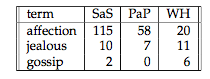
\includegraphics{terms.png}
\caption{novel terms}
\end{figure}

Such a matrix is also catted a Term-Document Matrix. Here, the terms
being indexed could be stemmed before indexing; for instance,
\texttt{jealous} and \texttt{jealousy} after stemming are the same
feature. One could also make use of other "Natural Language Processing"
transformations in constructing the vocabulary. We could use
Lemmatization, which reduces words to lemmas: work, working, worked
would all reduce to work. We could remove "stopwords" from our
vocabulary, such as common words like "the". We could look for
particular parts of speech, such as adjectives. This is often done in
Sentiment Analysis. And so on. It all depends on our application.

From the book: \textgreater{}The standard way of quantifying the
similarity between two documents \(d_1\) and \(d_2\) is to compute the
cosine similarity of their vector representations \(\bar V(d_1)\) and
\(\bar V(d_2)\):

\[S_{12} = \frac{\bar V(d_1) \cdot \bar V(d_2)}{|\bar V(d_1)| \times |\bar V(d_2)|}\]

\begin{figure}
\centering
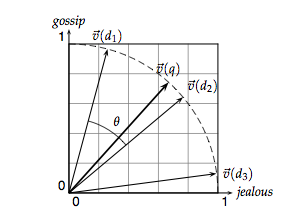
\includegraphics{vsm.png}
\caption{Vector Space Model}
\end{figure}

\begin{quote}
There is a far more compelling reason to represent documents as vectors:
we can also view a query as a vector. Consider the query q = jealous
gossip. This query turns into the unit vector \(\bar V(q)\) = (0, 0.707,
0.707) on the three coordinates below.
\end{quote}

\begin{figure}
\centering
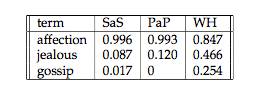
\includegraphics{terms2.png}
\caption{novel terms}
\end{figure}

\begin{quote}
The key idea now: to assign to each document d a score equal to the dot
product:
\end{quote}

\[\bar V(q) \cdot \bar V(d)\]

Then we can use this simple Vector Model as a Search engine.

    \subsubsection{In Code}\label{in-code}

    \begin{Verbatim}[commandchars=\\\{\}]
{\color{incolor}In [{\color{incolor}24}]:} \PY{k+kn}{from} \PY{n+nn}{sklearn}\PY{n+nn}{.}\PY{n+nn}{feature\PYZus{}extraction}\PY{n+nn}{.}\PY{n+nn}{text} \PY{k}{import} \PY{n}{CountVectorizer}
         
         \PY{n}{text} \PY{o}{=} \PY{p}{[}\PY{l+s+s1}{\PYZsq{}}\PY{l+s+s1}{Hop on pop}\PY{l+s+s1}{\PYZsq{}}\PY{p}{,} \PY{l+s+s1}{\PYZsq{}}\PY{l+s+s1}{Hop off pop}\PY{l+s+s1}{\PYZsq{}}\PY{p}{,} \PY{l+s+s1}{\PYZsq{}}\PY{l+s+s1}{Hop Hop hop}\PY{l+s+s1}{\PYZsq{}}\PY{p}{]}
         \PY{n+nb}{print}\PY{p}{(}\PY{l+s+s2}{\PYZdq{}}\PY{l+s+s2}{Original text is}\PY{l+s+se}{\PYZbs{}n}\PY{l+s+si}{\PYZob{}\PYZcb{}}\PY{l+s+s2}{\PYZdq{}}\PY{o}{.}\PY{n}{format}\PY{p}{(}\PY{l+s+s1}{\PYZsq{}}\PY{l+s+se}{\PYZbs{}n}\PY{l+s+s1}{\PYZsq{}}\PY{o}{.}\PY{n}{join}\PY{p}{(}\PY{n}{text}\PY{p}{)}\PY{p}{)}\PY{p}{)}
         
         \PY{n}{vectorizer} \PY{o}{=} \PY{n}{CountVectorizer}\PY{p}{(}\PY{n}{min\PYZus{}df}\PY{o}{=}\PY{l+m+mi}{0}\PY{p}{)}  \PY{c+c1}{\PYZsh{}instanciating to set the model}
         
         \PY{c+c1}{\PYZsh{} call `fit` to build the vocabulary}
         \PY{n}{vectorizer}\PY{o}{.}\PY{n}{fit}\PY{p}{(}\PY{n}{text}\PY{p}{)}
         
         \PY{c+c1}{\PYZsh{} call `transform` to convert text to a bag of words}
         \PY{n}{x} \PY{o}{=} \PY{n}{vectorizer}\PY{o}{.}\PY{n}{transform}\PY{p}{(}\PY{n}{text}\PY{p}{)}
         
         \PY{c+c1}{\PYZsh{} CountVectorizer uses a sparse array to save memory, but it\PYZsq{}s easier in this assignment to }
         \PY{c+c1}{\PYZsh{} convert back to a \PYZdq{}normal\PYZdq{} numpy array}
         \PY{n}{x} \PY{o}{=} \PY{n}{x}\PY{o}{.}\PY{n}{toarray}\PY{p}{(}\PY{p}{)}
         
         \PY{n+nb}{print}\PY{p}{(}\PY{l+s+s2}{\PYZdq{}}\PY{l+s+s2}{\PYZdq{}}\PY{p}{)}
         \PY{n+nb}{print}\PY{p}{(}\PY{l+s+s2}{\PYZdq{}}\PY{l+s+s2}{Transformed text vector is }\PY{l+s+se}{\PYZbs{}n}\PY{l+s+si}{\PYZob{}\PYZcb{}}\PY{l+s+s2}{\PYZdq{}}\PY{o}{.}\PY{n}{format}\PY{p}{(}\PY{n}{x}\PY{p}{)}\PY{p}{)}
         
         \PY{c+c1}{\PYZsh{} `get\PYZus{}feature\PYZus{}names` tracks which word is associated with each column of the transformed x}
         \PY{n+nb}{print}\PY{p}{(}\PY{l+s+s2}{\PYZdq{}}\PY{l+s+s2}{\PYZdq{}}\PY{p}{)}
         \PY{n+nb}{print}\PY{p}{(}\PY{l+s+s2}{\PYZdq{}}\PY{l+s+s2}{Words for each feature:}\PY{l+s+s2}{\PYZdq{}}\PY{p}{)}
         \PY{n+nb}{print}\PY{p}{(}\PY{n}{vectorizer}\PY{o}{.}\PY{n}{get\PYZus{}feature\PYZus{}names}\PY{p}{(}\PY{p}{)}\PY{p}{)}
         
         \PY{c+c1}{\PYZsh{} Notice that the bag of words treatment doesn\PYZsq{}t preserve information about the *order* of words, }
         \PY{c+c1}{\PYZsh{} just their frequency}
\end{Verbatim}


    \begin{Verbatim}[commandchars=\\\{\}]
Original text is
Hop on pop
Hop off pop
Hop Hop hop

Transformed text vector is 
[[1 0 1 1]
 [1 1 0 1]
 [3 0 0 0]]

Words for each feature:
['hop', 'off', 'on', 'pop']

    \end{Verbatim}

    \begin{Verbatim}[commandchars=\\\{\}]
{\color{incolor}In [{\color{incolor}25}]:} \PY{k}{def} \PY{n+nf}{make\PYZus{}xy}\PY{p}{(}\PY{n}{critics}\PY{p}{,} \PY{n}{vectorizer}\PY{o}{=}\PY{k+kc}{None}\PY{p}{)}\PY{p}{:} \PY{c+c1}{\PYZsh{}???}
             \PY{c+c1}{\PYZsh{}Your code here    }
             \PY{k}{if} \PY{n}{vectorizer} \PY{o+ow}{is} \PY{k+kc}{None}\PY{p}{:}
                 \PY{n}{vectorizer} \PY{o}{=} \PY{n}{CountVectorizer}\PY{p}{(}\PY{p}{)}
             \PY{n}{X} \PY{o}{=} \PY{n}{vectorizer}\PY{o}{.}\PY{n}{fit\PYZus{}transform}\PY{p}{(}\PY{n}{critics}\PY{o}{.}\PY{n}{quote}\PY{p}{)}
             \PY{n}{X} \PY{o}{=} \PY{n}{X}\PY{o}{.}\PY{n}{tocsc}\PY{p}{(}\PY{p}{)}  \PY{c+c1}{\PYZsh{} some versions of sklearn return COO format}
             \PY{n}{y} \PY{o}{=} \PY{p}{(}\PY{n}{critics}\PY{o}{.}\PY{n}{fresh} \PY{o}{==} \PY{l+s+s1}{\PYZsq{}}\PY{l+s+s1}{fresh}\PY{l+s+s1}{\PYZsq{}}\PY{p}{)}\PY{o}{.}\PY{n}{values}\PY{o}{.}\PY{n}{astype}\PY{p}{(}\PY{n}{np}\PY{o}{.}\PY{n}{int}\PY{p}{)} \PY{c+c1}{\PYZsh{}uses a logical to turn the fresh reviews into the number 1}
             \PY{k}{return} \PY{n}{X}\PY{p}{,} \PY{n}{y}
         \PY{n}{X}\PY{p}{,} \PY{n}{y} \PY{o}{=} \PY{n}{make\PYZus{}xy}\PY{p}{(}\PY{n}{critics}\PY{p}{)}
\end{Verbatim}


    \begin{Verbatim}[commandchars=\\\{\}]
{\color{incolor}In [{\color{incolor}28}]:} \PY{n+nb}{print}\PY{p}{(}\PY{n}{y}\PY{p}{)} \PY{c+c1}{\PYZsh{}each sentence is cooresponding with a fresh or rotten rating}
\end{Verbatim}


    \begin{Verbatim}[commandchars=\\\{\}]
[1 1 1 {\ldots} 1 1 1]

    \end{Verbatim}

    \subsection{Naive Bayes}\label{naive-bayes}

    From Bayes' Theorem, we have that

\[P(c \vert f) = \frac{P(c \cap f)}{P(f)}\]

where \(c\) represents a \emph{class} or category, and \(f\) represents
a feature vector, such as \(\bar V(d)\) as above. \textbf{We are
computing the probability that a document (or whatever we are
classifying) belongs to category \emph{c} given the features in the
document.} \(P(f)\) is really just a normalization constant, so the
literature usually writes Bayes' Theorem in context of Naive Bayes as

\[P(c \vert f) \propto P(f \vert c) P(c) \]

\(P(c)\) is called the \emph{prior} and is simply the probability of
seeing class \(c\). But what is \(P(f \vert c)\)? This is the
probability that we see feature set \(f\) given that this document is
actually in class \(c\). This is called the \emph{likelihood} and comes
from the data. One of the major assumptions of the Naive Bayes model is
that the features are \emph{conditionally independent} given the class.
While the presence of a particular discriminative word may uniquely
identify the document as being part of class \(c\) and thus violate
general feature independence, conditional independence means that the
presence of that term is independent of all the other words that appear
\emph{within that class}. This is a very important distinction. Recall
that if two events are independent, then:

\[P(A \cap B) = P(A) \cdot P(B)\]

Thus, conditional independence implies

\[P(f \vert c)  = \prod_i P(f_i | c) \]

where \(f_i\) is an individual feature (a word in this example).

To make a classification, we then choose the class \(c\) such that
\(P(c \vert f)\) is maximal.

There is a small caveat when computing these probabilities. For
\href{http://nlp.stanford.edu/IR-book/html/htmledition/naive-bayes-text-classification-1.html}{floating
point underflow} we change the product into a sum by going into log
space. This is called the LogSumExp trick. So:

\[\log P(f \vert c)  = \sum_i \log P(f_i \vert c) \]

There is another caveat. What if we see a term that didn't exist in the
training data? This means that \(P(f_i \vert c) = 0\) for that term, and
thus \(P(f \vert c) = \prod_i P(f_i | c) = 0\), which doesn't help us at
all. Instead of using zeros, we add a small negligible value called
\(\alpha\) to each count. This is called Laplace Smoothing.

\[P(f_i \vert c) = \frac{N_{ic}+\alpha}{N_c + \alpha N_i}\]

where \(N_{ic}\) is the number of times feature \(i\) was seen in class
\(c\), \(N_c\) is the number of times class \(c\) was seen and \(N_i\)
is the number of times feature \(i\) was seen globally. \(\alpha\) is
sometimes called a regularization parameter.

    \subsubsection{Multinomial Naive Bayes and Other Likelihood
Functions}\label{multinomial-naive-bayes-and-other-likelihood-functions}

Since we are modeling word counts, we are using variation of Naive Bayes
called Multinomial Naive Bayes. This is because the likelihood function
actually takes the form of the multinomial distribution.

\[P(f \vert c) = \frac{\left( \sum_i f_i \right)!}{\prod_i f_i!} \prod_{f_i} P(f_i \vert c)^{f_i} \propto \prod_{i} P(f_i \vert c)\]

where the nasty term out front is absorbed as a normalization constant
such that probabilities sum to 1.

There are many other variations of Naive Bayes, all which depend on what
type of value \(f_i\) takes. If \(f_i\) is continuous, we may be able to
use \emph{Gaussian Naive Bayes}. First compute the mean and variance for
each class \(c\). Then the likelihood, \(P(f \vert c)\) is given as
follows

\[P(f_i = v \vert c) = \frac{1}{\sqrt{2\pi \sigma^2_c}} e^{- \frac{\left( v - \mu_c \right)^2}{2 \sigma^2_c}}\]

    Exercise Set II

Exercise: Implement a simple Naive Bayes classifier:

split the data set into a training and test set

Use \texttt{scikit-learn}'s \texttt{MultinomialNB()} classifier with
default parameters.

train the classifier over the training set and test on the test set

print the accuracy scores for both the training and the test sets

What do you notice? Is this a good classifier? If not, why not?

    \begin{Verbatim}[commandchars=\\\{\}]
{\color{incolor}In [{\color{incolor}29}]:} \PY{c+c1}{\PYZsh{}your turn}
         
         \PY{k+kn}{from} \PY{n+nn}{sklearn}\PY{n+nn}{.}\PY{n+nn}{model\PYZus{}selection} \PY{k}{import} \PY{n}{train\PYZus{}test\PYZus{}split}
         \PY{k+kn}{from} \PY{n+nn}{sklearn}\PY{n+nn}{.}\PY{n+nn}{naive\PYZus{}bayes} \PY{k}{import} \PY{n}{MultinomialNB}
         \PY{n}{X\PYZus{}train}\PY{p}{,} \PY{n}{X\PYZus{}test}\PY{p}{,} \PY{n}{y\PYZus{}train}\PY{p}{,} \PY{n}{y\PYZus{}test} \PY{o}{=} \PY{n}{train\PYZus{}test\PYZus{}split}\PY{p}{(}\PY{n}{X}\PY{p}{,}\PY{n}{y}\PY{p}{,}\PY{n}{test\PYZus{}size}\PY{o}{=}\PY{l+m+mf}{0.7}\PY{p}{)}
         \PY{n}{classifier} \PY{o}{=} \PY{n}{MultinomialNB}\PY{p}{(}\PY{p}{)}
         
         \PY{n}{classifier}\PY{o}{.}\PY{n}{fit}\PY{p}{(}\PY{n}{X\PYZus{}train}\PY{p}{,}\PY{n}{y\PYZus{}train}\PY{p}{)}
         \PY{n}{classifier}\PY{o}{.}\PY{n}{predict}\PY{p}{(}\PY{n}{X\PYZus{}test}\PY{p}{)}
         \PY{n+nb}{print}\PY{p}{(}\PY{l+s+s2}{\PYZdq{}}\PY{l+s+s2}{Training accuracy is: }\PY{l+s+si}{\PYZpc{}.3f}\PY{l+s+si}{\PYZpc{}\PYZpc{}}\PY{l+s+s2}{ }\PY{l+s+s2}{\PYZdq{}} \PY{o}{\PYZpc{}} \PY{p}{(}\PY{n}{classifier}\PY{o}{.}\PY{n}{score}\PY{p}{(}\PY{n}{X\PYZus{}train}\PY{p}{,} \PY{n}{y\PYZus{}train}\PY{p}{)}\PY{o}{*}\PY{l+m+mi}{100}\PY{p}{)}\PY{p}{)}
         \PY{n+nb}{print}\PY{p}{(}\PY{l+s+s2}{\PYZdq{}}\PY{l+s+s2}{Testing accuracy is: }\PY{l+s+si}{\PYZpc{}.3f}\PY{l+s+si}{\PYZpc{}\PYZpc{}}\PY{l+s+s2}{\PYZdq{}} \PY{o}{\PYZpc{}} \PY{p}{(}\PY{n}{classifier}\PY{o}{.}\PY{n}{score}\PY{p}{(}\PY{n}{X\PYZus{}test}\PY{p}{,} \PY{n}{y\PYZus{}test}\PY{p}{)}\PY{o}{*}\PY{l+m+mi}{100}\PY{p}{)}\PY{p}{)}
\end{Verbatim}


    \begin{Verbatim}[commandchars=\\\{\}]
Training accuracy is: 92.309\% 
Testing accuracy is: 73.717\%

    \end{Verbatim}

    The model appears to be overfit. The testing accuracy is a bit lower
than the training one. All in all the model is fairly accurate though.

    \subsubsection{Picking Hyperparameters for Naive Bayes and Text
Maintenance}\label{picking-hyperparameters-for-naive-bayes-and-text-maintenance}

    We need to know what value to use for \(\alpha\), and we also need to
know which words to include in the vocabulary. As mentioned earlier,
some words are obvious stopwords. Other words appear so infrequently
that they serve as noise, and other words in addition to stopwords
appear so frequently that they may also serve as noise.

    First, let's find an appropriate value for \texttt{min\_df} for the
\texttt{CountVectorizer}. \texttt{min\_df} can be either an integer or a
float/decimal. If it is an integer, \texttt{min\_df} represents the
minimum number of documents a word must appear in for it to be included
in the vocabulary. If it is a float, it represents the minimum
\emph{percentage} of documents a word must appear in to be included in
the vocabulary. From the documentation:

    \begin{quote}
min\_df: When building the vocabulary ignore terms that have a document
frequency strictly lower than the given threshold. This value is also
called cut-off in the literature. If float, the parameter represents a
proportion of documents, integer absolute counts. This parameter is
ignored if vocabulary is not None.
\end{quote}

    Exercise Set III

Exercise: Construct the cumulative distribution of document frequencies
(df). The \(x\)-axis is a document count \(x_i\) and the \(y\)-axis is
the percentage of words that appear less than \(x_i\) times. For
example, at \(x=5\), plot a point representing the percentage or number
of words that appear in 5 or fewer documents.

Exercise: Look for the point at which the curve begins climbing steeply.
This may be a good value for \texttt{min\_df}. If we were interested in
also picking \texttt{max\_df}, we would likely pick the value where the
curve starts to plateau. What value did you choose?

    \begin{Verbatim}[commandchars=\\\{\}]
{\color{incolor}In [{\color{incolor}32}]:} \PY{c+c1}{\PYZsh{} Your turn.}
         \PY{n}{wordcount} \PY{o}{=} \PY{n}{vectorizer}\PY{o}{.}\PY{n}{fit\PYZus{}transform}\PY{p}{(}\PY{n}{critics}\PY{p}{[}\PY{l+s+s1}{\PYZsq{}}\PY{l+s+s1}{quote}\PY{l+s+s1}{\PYZsq{}}\PY{p}{]}\PY{p}{)} \PY{c+c1}{\PYZsh{}fitting and transforming it}
         \PY{n}{wordcountdf} \PY{o}{=} \PY{n}{pd}\PY{o}{.}\PY{n}{DataFrame}\PY{p}{(}\PY{n}{wordcount}\PY{o}{.}\PY{n}{toarray}\PY{p}{(}\PY{p}{)}\PY{p}{)} \PY{c+c1}{\PYZsh{}turning the quote column into an array, and then a pandas dataframe}
         \PY{n}{totals} \PY{o}{=} \PY{n}{wordcountdf}\PY{o}{.}\PY{n}{sum}\PY{p}{(}\PY{l+m+mi}{1}\PY{p}{)} \PY{c+c1}{\PYZsh{} 1 might be the axis}
         \PY{n}{sns}\PY{o}{.}\PY{n}{kdeplot}\PY{p}{(}\PY{n}{totals}\PY{p}{,} \PY{n}{cumulative}\PY{o}{=}\PY{k+kc}{True}\PY{p}{)} 
\end{Verbatim}


\begin{Verbatim}[commandchars=\\\{\}]
{\color{outcolor}Out[{\color{outcolor}32}]:} <matplotlib.axes.\_subplots.AxesSubplot at 0x13a3c323a20>
\end{Verbatim}
            
    \begin{center}
    \adjustimage{max size={0.9\linewidth}{0.9\paperheight}}{output_26_1.png}
    \end{center}
    { \hspace*{\fill} \\}
    
    \begin{Verbatim}[commandchars=\\\{\}]
{\color{incolor}In [{\color{incolor}22}]:} \PY{n+nb}{print}\PY{p}{(}\PY{n}{wordcount}\PY{p}{)}
\end{Verbatim}


    \begin{Verbatim}[commandchars=\\\{\}]
  (0, 3248)	1
  (0, 10566)	1
  (0, 2784)	1
  (0, 6494)	1
  (0, 1767)	1
  (0, 18904)	1
  (0, 17231)	1
  (0, 17943)	1
  (0, 18757)	1
  (0, 14940)	1
  (0, 13657)	1
  (0, 10555)	1
  (0, 21732)	1
  (0, 4386)	1
  (0, 22330)	1
  (0, 19914)	1
  (0, 6856)	1
  (0, 891)	2
  (0, 5251)	1
  (0, 4003)	1
  (0, 9950)	1
  (0, 10176)	1
  (0, 18252)	1
  (1, 3835)	1
  (1, 10463)	1
  :	:
  (15559, 19917)	3
  (15559, 10566)	1
  (15559, 18904)	1
  (15559, 19914)	1
  (15559, 891)	1
  (15560, 19057)	1
  (15560, 10261)	1
  (15560, 8719)	1
  (15560, 362)	1
  (15560, 5294)	1
  (15560, 6527)	1
  (15560, 5747)	1
  (15560, 15259)	1
  (15560, 20129)	1
  (15560, 9087)	1
  (15560, 10363)	1
  (15560, 11404)	1
  (15560, 21212)	1
  (15560, 10891)	1
  (15560, 20187)	1
  (15560, 13584)	1
  (15560, 7729)	1
  (15560, 19917)	2
  (15560, 10555)	1
  (15560, 891)	1

    \end{Verbatim}

    The curve begins climbing at about 3, and seems to plataeu at about 35

    The parameter \(\alpha\) is chosen to be a small value that simply
avoids having zeros in the probability computations. This value can
sometimes be chosen arbitrarily with domain expertise, but we will use
K-fold cross validation. In K-fold cross-validation, we divide the data
into \(K\) non-overlapping parts. We train on \(K-1\) of the folds and
test on the remaining fold. We then iterate, so that each fold serves as
the test fold exactly once. The function \texttt{cv\_score} performs the
K-fold cross-validation algorithm for us, but we need to pass a function
that measures the performance of the algorithm on each fold.

    \begin{Verbatim}[commandchars=\\\{\}]
{\color{incolor}In [{\color{incolor}9}]:} \PY{k+kn}{from} \PY{n+nn}{sklearn}\PY{n+nn}{.}\PY{n+nn}{model\PYZus{}selection} \PY{k}{import} \PY{n}{KFold}
        \PY{k}{def} \PY{n+nf}{cv\PYZus{}score}\PY{p}{(}\PY{n}{clf}\PY{p}{,} \PY{n}{X}\PY{p}{,} \PY{n}{y}\PY{p}{,} \PY{n}{scorefunc}\PY{p}{)}\PY{p}{:} \PY{c+c1}{\PYZsh{} isn\PYZsq{}t there already a module to do cv\PYZus{}score?}
            \PY{n}{result} \PY{o}{=} \PY{l+m+mf}{0.}
            \PY{n}{nfold} \PY{o}{=} \PY{l+m+mi}{5}
            \PY{k}{for} \PY{n}{train}\PY{p}{,} \PY{n}{test} \PY{o+ow}{in} \PY{n}{KFold}\PY{p}{(}\PY{n}{nfold}\PY{p}{)}\PY{o}{.}\PY{n}{split}\PY{p}{(}\PY{n}{X}\PY{p}{)}\PY{p}{:} \PY{c+c1}{\PYZsh{} split data into train/test groups, 5 times}
                \PY{n}{clf}\PY{o}{.}\PY{n}{fit}\PY{p}{(}\PY{n}{X}\PY{p}{[}\PY{n}{train}\PY{p}{]}\PY{p}{,} \PY{n}{y}\PY{p}{[}\PY{n}{train}\PY{p}{]}\PY{p}{)} \PY{c+c1}{\PYZsh{} fit the classifier, passed is as clf.}
                \PY{n}{result} \PY{o}{+}\PY{o}{=} \PY{n}{scorefunc}\PY{p}{(}\PY{n}{clf}\PY{p}{,} \PY{n}{X}\PY{p}{[}\PY{n}{test}\PY{p}{]}\PY{p}{,} \PY{n}{y}\PY{p}{[}\PY{n}{test}\PY{p}{]}\PY{p}{)} \PY{c+c1}{\PYZsh{} evaluate score function on held\PYZhy{}out data}
            \PY{k}{return} \PY{n}{result} \PY{o}{/} \PY{n}{nfold} \PY{c+c1}{\PYZsh{} average \PYZsh{}???}
\end{Verbatim}


    We use the log-likelihood as the score here in \texttt{scorefunc}. The
higher the log-likelihood, the better. Indeed, what we do in
\texttt{cv\_score} above is to implement the cross-validation part of
\texttt{GridSearchCV}.

The custom scoring function \texttt{scorefunc} allows us to use
different metrics depending on the decision risk we care about
(precision, accuracy, profit etc.) directly on the validation set. You
will often find people using \texttt{roc\_auc}, precision, recall, or
\texttt{F1-score} as the scoring function.

    \begin{Verbatim}[commandchars=\\\{\}]
{\color{incolor}In [{\color{incolor}10}]:} \PY{k}{def} \PY{n+nf}{log\PYZus{}likelihood}\PY{p}{(}\PY{n}{clf}\PY{p}{,} \PY{n}{x}\PY{p}{,} \PY{n}{y}\PY{p}{)}\PY{p}{:}
             \PY{n}{prob} \PY{o}{=} \PY{n}{clf}\PY{o}{.}\PY{n}{predict\PYZus{}log\PYZus{}proba}\PY{p}{(}\PY{n}{x}\PY{p}{)}
             \PY{n}{rotten} \PY{o}{=} \PY{n}{y} \PY{o}{==} \PY{l+m+mi}{0}
             \PY{n}{fresh} \PY{o}{=} \PY{o}{\PYZti{}}\PY{n}{rotten}
             \PY{k}{return} \PY{n}{prob}\PY{p}{[}\PY{n}{rotten}\PY{p}{,} \PY{l+m+mi}{0}\PY{p}{]}\PY{o}{.}\PY{n}{sum}\PY{p}{(}\PY{p}{)} \PY{o}{+} \PY{n}{prob}\PY{p}{[}\PY{n}{fresh}\PY{p}{,} \PY{l+m+mi}{1}\PY{p}{]}\PY{o}{.}\PY{n}{sum}\PY{p}{(}\PY{p}{)}
\end{Verbatim}


    We'll cross-validate over the regularization parameter \(\alpha\).

    Let's set up the train and test masks first, and then we can run the
cross-validation procedure.

    \begin{Verbatim}[commandchars=\\\{\}]
{\color{incolor}In [{\color{incolor}40}]:} \PY{k+kn}{from} \PY{n+nn}{sklearn}\PY{n+nn}{.}\PY{n+nn}{model\PYZus{}selection} \PY{k}{import} \PY{n}{train\PYZus{}test\PYZus{}split}
         \PY{n}{\PYZus{}}\PY{p}{,} \PY{n}{itest} \PY{o}{=} \PY{n}{train\PYZus{}test\PYZus{}split}\PY{p}{(}\PY{n+nb}{range}\PY{p}{(}\PY{n}{critics}\PY{o}{.}\PY{n}{shape}\PY{p}{[}\PY{l+m+mi}{0}\PY{p}{]}\PY{p}{)}\PY{p}{,} \PY{n}{train\PYZus{}size}\PY{o}{=}\PY{l+m+mf}{0.7}\PY{p}{)} \PY{c+c1}{\PYZsh{}???}
         \PY{n}{mask} \PY{o}{=} \PY{n}{np}\PY{o}{.}\PY{n}{zeros}\PY{p}{(}\PY{n}{critics}\PY{o}{.}\PY{n}{shape}\PY{p}{[}\PY{l+m+mi}{0}\PY{p}{]}\PY{p}{,} \PY{n}{dtype}\PY{o}{=}\PY{n}{np}\PY{o}{.}\PY{n}{bool}\PY{p}{)} \PY{c+c1}{\PYZsh{}makes an empty array filled with 0 the same size as the array of interest, making sure its a boolean}
         \PY{n}{mask}\PY{p}{[}\PY{n}{itest}\PY{p}{]} \PY{o}{=} \PY{k+kc}{True}
\end{Verbatim}


    \begin{Verbatim}[commandchars=\\\{\}]
C:\textbackslash{}Users\textbackslash{}Ameen\textbackslash{}Miniconda3\textbackslash{}lib\textbackslash{}site-packages\textbackslash{}sklearn\textbackslash{}model\_selection\textbackslash{}\_split.py:2026: FutureWarning: From version 0.21, test\_size will always complement train\_size unless both are specified.
  FutureWarning)

    \end{Verbatim}

    \begin{Verbatim}[commandchars=\\\{\}]
{\color{incolor}In [{\color{incolor}39}]:} \PY{n+nb}{print}\PY{p}{(}\PY{n}{critics}\PY{o}{.}\PY{n}{shape}\PY{p}{)}
\end{Verbatim}


    \begin{Verbatim}[commandchars=\\\{\}]
(15561, 8)

    \end{Verbatim}

    Exercise Set IV

Exercise: What does using the function \texttt{log\_likelihood} as the
score mean? What are we trying to optimize for?

Exercise: Without writing any code, what do you think would happen if
you choose a value of \(\alpha\) that is too high?

Exercise: Using the skeleton code below, find the best values of the
parameter \texttt{alpha}, and use the value of \texttt{min\_df} you
chose in the previous exercise set. Use the \texttt{cv\_score} function
above with the \texttt{log\_likelihood} function for scoring.

It is the sum of all the probabilities of the model correctly predicting
the parameter, rotten / fresh. It is adding the two together. The higher
this is, the better the model is doing. We are trying to optimize the
hyperparamaters so the accuracy is higher.

I imagine a higher alpha would make the model less accurate.

    \begin{Verbatim}[commandchars=\\\{\}]
{\color{incolor}In [{\color{incolor}12}]:} \PY{k+kn}{from} \PY{n+nn}{sklearn}\PY{n+nn}{.}\PY{n+nn}{naive\PYZus{}bayes} \PY{k}{import} \PY{n}{MultinomialNB}
         
         \PY{c+c1}{\PYZsh{}the grid of parameters to search over}
         \PY{n}{alphas} \PY{o}{=} \PY{p}{[}\PY{o}{.}\PY{l+m+mi}{1}\PY{p}{,} \PY{l+m+mi}{1}\PY{p}{,} \PY{l+m+mi}{5}\PY{p}{,} \PY{l+m+mi}{10}\PY{p}{,} \PY{l+m+mi}{50}\PY{p}{]}
         \PY{n}{best\PYZus{}min\PYZus{}df} \PY{o}{=} \PY{l+m+mi}{3} \PY{c+c1}{\PYZsh{} YOUR TURN: put your value of min\PYZus{}df here.}
         
         \PY{c+c1}{\PYZsh{}Find the best value for alpha and min\PYZus{}df, and the best classifier}
         \PY{n}{best\PYZus{}alpha} \PY{o}{=} \PY{l+m+mi}{1}
         \PY{n}{maxscore}\PY{o}{=}\PY{o}{\PYZhy{}}\PY{n}{np}\PY{o}{.}\PY{n}{inf}
         \PY{k}{for} \PY{n}{alpha} \PY{o+ow}{in} \PY{n}{alphas}\PY{p}{:}        
             \PY{n}{vectorizer} \PY{o}{=} \PY{n}{CountVectorizer}\PY{p}{(}\PY{n}{min\PYZus{}df}\PY{o}{=}\PY{n}{best\PYZus{}min\PYZus{}df}\PY{p}{)}       
             \PY{n}{Xthis}\PY{p}{,} \PY{n}{ythis} \PY{o}{=} \PY{n}{make\PYZus{}xy}\PY{p}{(}\PY{n}{critics}\PY{p}{,} \PY{n}{vectorizer}\PY{p}{)}
             \PY{n}{Xtrainthis} \PY{o}{=} \PY{n}{Xthis}\PY{p}{[}\PY{n}{mask}\PY{p}{]}
             \PY{n}{ytrainthis} \PY{o}{=} \PY{n}{ythis}\PY{p}{[}\PY{n}{mask}\PY{p}{]}
             \PY{c+c1}{\PYZsh{} your turn}
             \PY{n}{clf} \PY{o}{=} \PY{n}{MultinomialNB}\PY{p}{(}\PY{n}{alpha}\PY{o}{=}\PY{n}{alpha}\PY{p}{)}
             \PY{n+nb}{print}\PY{p}{(}\PY{n}{alpha}\PY{p}{,} \PY{n}{cv\PYZus{}score}\PY{p}{(}\PY{n}{clf}\PY{p}{,} \PY{n}{Xtrainthis}\PY{p}{,} \PY{n}{ytrainthis}\PY{p}{,} \PY{n}{log\PYZus{}likelihood}\PY{p}{)}\PY{p}{)}
\end{Verbatim}


    \begin{Verbatim}[commandchars=\\\{\}]
0.1 -939.1108748884523
1 -590.6139511944126
5 -900.718147602239
10 -1152.9919534620046
50 -1328.7432612676503

    \end{Verbatim}

    \begin{Verbatim}[commandchars=\\\{\}]
{\color{incolor}In [{\color{incolor}13}]:} \PY{n+nb}{print}\PY{p}{(}\PY{l+s+s2}{\PYZdq{}}\PY{l+s+s2}{alpha: }\PY{l+s+si}{\PYZob{}\PYZcb{}}\PY{l+s+s2}{\PYZdq{}}\PY{o}{.}\PY{n}{format}\PY{p}{(}\PY{n}{best\PYZus{}alpha}\PY{p}{)}\PY{p}{)} \PY{c+c1}{\PYZsh{} with an alpha of 1, the log likelihood score was the highest}
\end{Verbatim}


    \begin{Verbatim}[commandchars=\\\{\}]
alpha: 1

    \end{Verbatim}

    Exercise Set V: Working with the Best Parameters

Exercise: Using the best value of \texttt{alpha} you just found,
calculate the accuracy on the training and test sets. Is this classifier
better? Why (not)?

    \begin{Verbatim}[commandchars=\\\{\}]
{\color{incolor}In [{\color{incolor}14}]:} \PY{n}{vectorizer} \PY{o}{=} \PY{n}{CountVectorizer}\PY{p}{(}\PY{n}{min\PYZus{}df}\PY{o}{=}\PY{n}{best\PYZus{}min\PYZus{}df}\PY{p}{)}
         \PY{n}{X}\PY{p}{,} \PY{n}{y} \PY{o}{=} \PY{n}{make\PYZus{}xy}\PY{p}{(}\PY{n}{critics}\PY{p}{,} \PY{n}{vectorizer}\PY{p}{)}
         \PY{n}{xtrain}\PY{o}{=}\PY{n}{X}\PY{p}{[}\PY{n}{mask}\PY{p}{]}
         \PY{n}{ytrain}\PY{o}{=}\PY{n}{y}\PY{p}{[}\PY{n}{mask}\PY{p}{]}
         \PY{n}{xtest}\PY{o}{=}\PY{n}{X}\PY{p}{[}\PY{o}{\PYZti{}}\PY{n}{mask}\PY{p}{]}
         \PY{n}{ytest}\PY{o}{=}\PY{n}{y}\PY{p}{[}\PY{o}{\PYZti{}}\PY{n}{mask}\PY{p}{]}
         
         \PY{n}{clf} \PY{o}{=} \PY{n}{MultinomialNB}\PY{p}{(}\PY{n}{alpha}\PY{o}{=}\PY{n}{best\PYZus{}alpha}\PY{p}{)}\PY{o}{.}\PY{n}{fit}\PY{p}{(}\PY{n}{xtrain}\PY{p}{,} \PY{n}{ytrain}\PY{p}{)}
         
         \PY{c+c1}{\PYZsh{}your turn. Print the accuracy on the test and training dataset}
         \PY{n}{training\PYZus{}accuracy} \PY{o}{=} \PY{n}{clf}\PY{o}{.}\PY{n}{score}\PY{p}{(}\PY{n}{xtrain}\PY{p}{,} \PY{n}{ytrain}\PY{p}{)}
         \PY{n}{test\PYZus{}accuracy} \PY{o}{=} \PY{n}{clf}\PY{o}{.}\PY{n}{score}\PY{p}{(}\PY{n}{xtest}\PY{p}{,} \PY{n}{ytest}\PY{p}{)}
         
         \PY{n+nb}{print}\PY{p}{(}\PY{l+s+s2}{\PYZdq{}}\PY{l+s+s2}{Accuracy on training data: }\PY{l+s+si}{\PYZob{}:2f\PYZcb{}}\PY{l+s+s2}{\PYZdq{}}\PY{o}{.}\PY{n}{format}\PY{p}{(}\PY{n}{training\PYZus{}accuracy}\PY{p}{)}\PY{p}{)}
         \PY{n+nb}{print}\PY{p}{(}\PY{l+s+s2}{\PYZdq{}}\PY{l+s+s2}{Accuracy on test data:     }\PY{l+s+si}{\PYZob{}:2f\PYZcb{}}\PY{l+s+s2}{\PYZdq{}}\PY{o}{.}\PY{n}{format}\PY{p}{(}\PY{n}{test\PYZus{}accuracy}\PY{p}{)}\PY{p}{)}
\end{Verbatim}


    \begin{Verbatim}[commandchars=\\\{\}]
Accuracy on training data: 0.928893
Accuracy on test data:     0.741462

    \end{Verbatim}

    old training score :91.99\% old testing score :77.13\%

The training score improved, but the testing score did not.

The huge difference between the Training Accuracy and the Test Accuracy
means that the model is still overfitting despite cross-validating in
order to choose alpha. Therefore, this classifier is not better in that
sense.

Attempt to cross-validate with a larger array of potential alphas may
improve the model and therefore improve the training and test
accuracies.

    \begin{Verbatim}[commandchars=\\\{\}]
{\color{incolor}In [{\color{incolor}15}]:} \PY{k+kn}{from} \PY{n+nn}{sklearn}\PY{n+nn}{.}\PY{n+nn}{metrics} \PY{k}{import} \PY{n}{confusion\PYZus{}matrix}
         \PY{n+nb}{print}\PY{p}{(}\PY{n}{confusion\PYZus{}matrix}\PY{p}{(}\PY{n}{ytest}\PY{p}{,} \PY{n}{clf}\PY{o}{.}\PY{n}{predict}\PY{p}{(}\PY{n}{xtest}\PY{p}{)}\PY{p}{)}\PY{p}{)}
\end{Verbatim}


    \begin{Verbatim}[commandchars=\\\{\}]
[[2525 1747]
 [1069 5551]]

    \end{Verbatim}

    \subsection{Interpretation}\label{interpretation}

    \subsubsection{What are the strongly predictive
features?}\label{what-are-the-strongly-predictive-features}

We use a neat trick to identify strongly predictive features (i.e.
words).

\begin{itemize}
\tightlist
\item
  first, create a data set such that each row has exactly one feature.
  This is represented by the identity matrix.
\item
  use the trained classifier to make predictions on this matrix
\item
  sort the rows by predicted probabilities, and pick the top and bottom
  \(K\) rows
\end{itemize}

    \begin{Verbatim}[commandchars=\\\{\}]
{\color{incolor}In [{\color{incolor}16}]:} \PY{n}{words} \PY{o}{=} \PY{n}{np}\PY{o}{.}\PY{n}{array}\PY{p}{(}\PY{n}{vectorizer}\PY{o}{.}\PY{n}{get\PYZus{}feature\PYZus{}names}\PY{p}{(}\PY{p}{)}\PY{p}{)}
         
         \PY{n}{x} \PY{o}{=} \PY{n}{np}\PY{o}{.}\PY{n}{eye}\PY{p}{(}\PY{n}{xtest}\PY{o}{.}\PY{n}{shape}\PY{p}{[}\PY{l+m+mi}{1}\PY{p}{]}\PY{p}{)}
         \PY{n}{probs} \PY{o}{=} \PY{n}{clf}\PY{o}{.}\PY{n}{predict\PYZus{}log\PYZus{}proba}\PY{p}{(}\PY{n}{x}\PY{p}{)}\PY{p}{[}\PY{p}{:}\PY{p}{,} \PY{l+m+mi}{0}\PY{p}{]}
         \PY{n}{ind} \PY{o}{=} \PY{n}{np}\PY{o}{.}\PY{n}{argsort}\PY{p}{(}\PY{n}{probs}\PY{p}{)}
         
         \PY{n}{good\PYZus{}words} \PY{o}{=} \PY{n}{words}\PY{p}{[}\PY{n}{ind}\PY{p}{[}\PY{p}{:}\PY{l+m+mi}{10}\PY{p}{]}\PY{p}{]}
         \PY{n}{bad\PYZus{}words} \PY{o}{=} \PY{n}{words}\PY{p}{[}\PY{n}{ind}\PY{p}{[}\PY{o}{\PYZhy{}}\PY{l+m+mi}{10}\PY{p}{:}\PY{p}{]}\PY{p}{]}
         
         \PY{n}{good\PYZus{}prob} \PY{o}{=} \PY{n}{probs}\PY{p}{[}\PY{n}{ind}\PY{p}{[}\PY{p}{:}\PY{l+m+mi}{10}\PY{p}{]}\PY{p}{]}
         \PY{n}{bad\PYZus{}prob} \PY{o}{=} \PY{n}{probs}\PY{p}{[}\PY{n}{ind}\PY{p}{[}\PY{o}{\PYZhy{}}\PY{l+m+mi}{10}\PY{p}{:}\PY{p}{]}\PY{p}{]}
         
         \PY{n+nb}{print}\PY{p}{(}\PY{l+s+s2}{\PYZdq{}}\PY{l+s+s2}{Good words}\PY{l+s+se}{\PYZbs{}t}\PY{l+s+s2}{     P(fresh | word)}\PY{l+s+s2}{\PYZdq{}}\PY{p}{)}
         \PY{k}{for} \PY{n}{w}\PY{p}{,} \PY{n}{p} \PY{o+ow}{in} \PY{n+nb}{zip}\PY{p}{(}\PY{n}{good\PYZus{}words}\PY{p}{,} \PY{n}{good\PYZus{}prob}\PY{p}{)}\PY{p}{:}
             \PY{n+nb}{print}\PY{p}{(}\PY{l+s+s2}{\PYZdq{}}\PY{l+s+si}{\PYZob{}:\PYZgt{}20\PYZcb{}}\PY{l+s+s2}{\PYZdq{}}\PY{o}{.}\PY{n}{format}\PY{p}{(}\PY{n}{w}\PY{p}{)}\PY{p}{,} \PY{l+s+s2}{\PYZdq{}}\PY{l+s+si}{\PYZob{}:.2f\PYZcb{}}\PY{l+s+s2}{\PYZdq{}}\PY{o}{.}\PY{n}{format}\PY{p}{(}\PY{l+m+mi}{1} \PY{o}{\PYZhy{}} \PY{n}{np}\PY{o}{.}\PY{n}{exp}\PY{p}{(}\PY{n}{p}\PY{p}{)}\PY{p}{)}\PY{p}{)}
             
         \PY{n+nb}{print}\PY{p}{(}\PY{l+s+s2}{\PYZdq{}}\PY{l+s+s2}{Bad words}\PY{l+s+se}{\PYZbs{}t}\PY{l+s+s2}{     P(fresh | word)}\PY{l+s+s2}{\PYZdq{}}\PY{p}{)}
         \PY{k}{for} \PY{n}{w}\PY{p}{,} \PY{n}{p} \PY{o+ow}{in} \PY{n+nb}{zip}\PY{p}{(}\PY{n}{bad\PYZus{}words}\PY{p}{,} \PY{n}{bad\PYZus{}prob}\PY{p}{)}\PY{p}{:}
             \PY{n+nb}{print}\PY{p}{(}\PY{l+s+s2}{\PYZdq{}}\PY{l+s+si}{\PYZob{}:\PYZgt{}20\PYZcb{}}\PY{l+s+s2}{\PYZdq{}}\PY{o}{.}\PY{n}{format}\PY{p}{(}\PY{n}{w}\PY{p}{)}\PY{p}{,} \PY{l+s+s2}{\PYZdq{}}\PY{l+s+si}{\PYZob{}:.2f\PYZcb{}}\PY{l+s+s2}{\PYZdq{}}\PY{o}{.}\PY{n}{format}\PY{p}{(}\PY{l+m+mi}{1} \PY{o}{\PYZhy{}} \PY{n}{np}\PY{o}{.}\PY{n}{exp}\PY{p}{(}\PY{n}{p}\PY{p}{)}\PY{p}{)}\PY{p}{)}
\end{Verbatim}


    \begin{Verbatim}[commandchars=\\\{\}]
Good words	     P(fresh | word)
         beautifully 0.96
               witty 0.96
              detail 0.96
                rare 0.96
            touching 0.95
             delight 0.94
         intelligent 0.94
       extraordinary 0.94
         achievement 0.94
         brilliantly 0.94
Bad words	     P(fresh | word)
                poor 0.12
            sluggish 0.12
            overlong 0.12
             unfunny 0.11
               sadly 0.11
          uninspired 0.10
           halloween 0.10
                lame 0.10
       unfortunately 0.08
           pointless 0.08

    \end{Verbatim}

    Exercise Set VI

Exercise: Why does this method work? What does the probability for each
row in the identity matrix represent

The probability represents the liklihood of a review receving a fresh or
rotten scoring, given that the review containe said word, or feature.

    The above exercise is an example of \emph{feature selection}. There are
many other feature selection methods. A list of feature selection
methods available in \texttt{sklearn} is
\href{http://scikit-learn.org/stable/modules/classes.html\#module-sklearn.feature_selection}{here}.
The most common feature selection technique for text mining is the
chi-squared \(\left( \chi^2 \right)\)
\href{http://nlp.stanford.edu/IR-book/html/htmledition/feature-selectionchi2-feature-selection-1.html}{method}.

    \subsubsection{Prediction Errors}\label{prediction-errors}

We can see mis-predictions as well.

    \begin{Verbatim}[commandchars=\\\{\}]
{\color{incolor}In [{\color{incolor}17}]:} \PY{n}{x}\PY{p}{,} \PY{n}{y} \PY{o}{=} \PY{n}{make\PYZus{}xy}\PY{p}{(}\PY{n}{critics}\PY{p}{,} \PY{n}{vectorizer}\PY{p}{)}
         
         \PY{n}{prob} \PY{o}{=} \PY{n}{clf}\PY{o}{.}\PY{n}{predict\PYZus{}proba}\PY{p}{(}\PY{n}{x}\PY{p}{)}\PY{p}{[}\PY{p}{:}\PY{p}{,} \PY{l+m+mi}{0}\PY{p}{]}
         \PY{n}{predict} \PY{o}{=} \PY{n}{clf}\PY{o}{.}\PY{n}{predict}\PY{p}{(}\PY{n}{x}\PY{p}{)}
         
         \PY{n}{bad\PYZus{}rotten} \PY{o}{=} \PY{n}{np}\PY{o}{.}\PY{n}{argsort}\PY{p}{(}\PY{n}{prob}\PY{p}{[}\PY{n}{y} \PY{o}{==} \PY{l+m+mi}{0}\PY{p}{]}\PY{p}{)}\PY{p}{[}\PY{p}{:}\PY{l+m+mi}{5}\PY{p}{]}
         \PY{n}{bad\PYZus{}fresh} \PY{o}{=} \PY{n}{np}\PY{o}{.}\PY{n}{argsort}\PY{p}{(}\PY{n}{prob}\PY{p}{[}\PY{n}{y} \PY{o}{==} \PY{l+m+mi}{1}\PY{p}{]}\PY{p}{)}\PY{p}{[}\PY{o}{\PYZhy{}}\PY{l+m+mi}{5}\PY{p}{:}\PY{p}{]}
         
         \PY{n+nb}{print}\PY{p}{(}\PY{l+s+s2}{\PYZdq{}}\PY{l+s+s2}{Mis\PYZhy{}predicted Rotten quotes}\PY{l+s+s2}{\PYZdq{}}\PY{p}{)}
         \PY{n+nb}{print}\PY{p}{(}\PY{l+s+s1}{\PYZsq{}}\PY{l+s+s1}{\PYZhy{}\PYZhy{}\PYZhy{}\PYZhy{}\PYZhy{}\PYZhy{}\PYZhy{}\PYZhy{}\PYZhy{}\PYZhy{}\PYZhy{}\PYZhy{}\PYZhy{}\PYZhy{}\PYZhy{}\PYZhy{}\PYZhy{}\PYZhy{}\PYZhy{}\PYZhy{}\PYZhy{}\PYZhy{}\PYZhy{}\PYZhy{}\PYZhy{}\PYZhy{}\PYZhy{}}\PY{l+s+s1}{\PYZsq{}}\PY{p}{)}
         \PY{k}{for} \PY{n}{row} \PY{o+ow}{in} \PY{n}{bad\PYZus{}rotten}\PY{p}{:}
             \PY{n+nb}{print}\PY{p}{(}\PY{n}{critics}\PY{p}{[}\PY{n}{y} \PY{o}{==} \PY{l+m+mi}{0}\PY{p}{]}\PY{o}{.}\PY{n}{quote}\PY{o}{.}\PY{n}{iloc}\PY{p}{[}\PY{n}{row}\PY{p}{]}\PY{p}{)}
             \PY{n+nb}{print}\PY{p}{(}\PY{l+s+s2}{\PYZdq{}}\PY{l+s+s2}{\PYZdq{}}\PY{p}{)}
         
         \PY{n+nb}{print}\PY{p}{(}\PY{l+s+s2}{\PYZdq{}}\PY{l+s+s2}{Mis\PYZhy{}predicted Fresh quotes}\PY{l+s+s2}{\PYZdq{}}\PY{p}{)}
         \PY{n+nb}{print}\PY{p}{(}\PY{l+s+s1}{\PYZsq{}}\PY{l+s+s1}{\PYZhy{}\PYZhy{}\PYZhy{}\PYZhy{}\PYZhy{}\PYZhy{}\PYZhy{}\PYZhy{}\PYZhy{}\PYZhy{}\PYZhy{}\PYZhy{}\PYZhy{}\PYZhy{}\PYZhy{}\PYZhy{}\PYZhy{}\PYZhy{}\PYZhy{}\PYZhy{}\PYZhy{}\PYZhy{}\PYZhy{}\PYZhy{}\PYZhy{}\PYZhy{}}\PY{l+s+s1}{\PYZsq{}}\PY{p}{)}
         \PY{k}{for} \PY{n}{row} \PY{o+ow}{in} \PY{n}{bad\PYZus{}fresh}\PY{p}{:}
             \PY{n+nb}{print}\PY{p}{(}\PY{n}{critics}\PY{p}{[}\PY{n}{y} \PY{o}{==} \PY{l+m+mi}{1}\PY{p}{]}\PY{o}{.}\PY{n}{quote}\PY{o}{.}\PY{n}{iloc}\PY{p}{[}\PY{n}{row}\PY{p}{]}\PY{p}{)}
             \PY{n+nb}{print}\PY{p}{(}\PY{l+s+s2}{\PYZdq{}}\PY{l+s+s2}{\PYZdq{}}\PY{p}{)}
\end{Verbatim}


    \begin{Verbatim}[commandchars=\\\{\}]
Mis-predicted Rotten quotes
---------------------------
It survives today only as an unusually pure example of a typical 50s art-film strategy: the attempt to make the most modern and most popular of art forms acceptable to the intelligentsia by forcing it into an arcane, antique mold.

It's not the actors' fault that no one is able to break through the film's gorgeous but chilly surface. You watch Casino with respect and appreciation, reveling in its documentary sense of detail.

While Leone's vision still has a magnificent sweep, the film finally subsides to an emotional core that is sombre, even elegiac, and which centres on a man who is bent and broken by time, and finally left with nothing but an impotent sadness.

Despite great scenery, the distinctive visual ideas of Mr. Scott (Alien, Blade Runner) and the strong dramatic presence of Mr. Bridges, most of White Squall remains listless and tame.

Walken is one of the few undeniably charismatic male villains of recent years; he can generate a snakelike charm that makes his worst characters the most memorable, and here he operates on pure style.

Mis-predicted Fresh quotes
--------------------------
[The scenes involving fire] are so good they make me recommend the movie anyway, despite its brain-damaged screenplay.

I saw this at a festival and hated it, then sat through it again a year later and decided it wasn't so bad, aside from the god-awful ending.

Considering the recent screen standards in book musicals with five numbers for 100 to 110 minutes of running time this Metro Santaclausing of numbers becomes virtually a double-feature filmusical.

Though it's a good half hour too long, this overblown 1993 spin-off of the 60s TV show otherwise adds up to a pretty good suspense thriller.

Consider this the big-screen equivalent of a beach read: Just turn off your brain and wallow in whatever turn-ons -- Whoopi and whoopee -- Stella offers.


    \end{Verbatim}

    Exercise Set VII: Predicting the Freshness for a New Review

Exercise:

Using your best trained classifier, predict the freshness of the
following sentence: \emph{'This movie is not remarkable, touching, or
superb in any way'}

Is the result what you'd expect? Why (not)?

    \begin{Verbatim}[commandchars=\\\{\}]
{\color{incolor}In [{\color{incolor}18}]:} \PY{c+c1}{\PYZsh{}your turn}
\end{Verbatim}


    \subsubsection{Aside: TF-IDF Weighting for Term
Importance}\label{aside-tf-idf-weighting-for-term-importance}

TF-IDF stands for

\texttt{Term-Frequency\ X\ Inverse\ Document\ Frequency}.

In the standard \texttt{CountVectorizer} model above, we used just the
term frequency in a document of words in our vocabulary. In TF-IDF, we
weight this term frequency by the inverse of its popularity in all
documents. For example, if the word "movie" showed up in all the
documents, it would not have much predictive value. It could actually be
considered a stopword. By weighing its counts by 1 divided by its
overall frequency, we downweight it. We can then use this TF-IDF
weighted features as inputs to any classifier. \textbf{TF-IDF is
essentially a measure of term importance, and of how discriminative a
word is in a corpus.} There are a variety of nuances involved in
computing TF-IDF, mainly involving where to add the smoothing term to
avoid division by 0, or log of 0 errors. The formula for TF-IDF in
\texttt{scikit-learn} differs from that of most textbooks:

\[\mbox{TF-IDF}(t, d) = \mbox{TF}(t, d)\times \mbox{IDF}(t) = n_{td} \log{\left( \frac{\vert D \vert}{\vert d : t \in d \vert} + 1 \right)}\]

where \(n_{td}\) is the number of times term \(t\) occurs in document
\(d\), \(\vert D \vert\) is the number of documents, and
\(\vert d : t \in d \vert\) is the number of documents that contain
\(t\)

    \begin{Verbatim}[commandchars=\\\{\}]
{\color{incolor}In [{\color{incolor}19}]:} \PY{c+c1}{\PYZsh{} http://scikit\PYZhy{}learn.org/dev/modules/feature\PYZus{}extraction.html\PYZsh{}text\PYZhy{}feature\PYZhy{}extraction}
         \PY{c+c1}{\PYZsh{} http://scikit\PYZhy{}learn.org/dev/modules/classes.html\PYZsh{}text\PYZhy{}feature\PYZhy{}extraction\PYZhy{}ref}
         \PY{k+kn}{from} \PY{n+nn}{sklearn}\PY{n+nn}{.}\PY{n+nn}{feature\PYZus{}extraction}\PY{n+nn}{.}\PY{n+nn}{text} \PY{k}{import} \PY{n}{TfidfVectorizer}
         \PY{n}{tfidfvectorizer} \PY{o}{=} \PY{n}{TfidfVectorizer}\PY{p}{(}\PY{n}{min\PYZus{}df}\PY{o}{=}\PY{l+m+mi}{1}\PY{p}{,} \PY{n}{stop\PYZus{}words}\PY{o}{=}\PY{l+s+s1}{\PYZsq{}}\PY{l+s+s1}{english}\PY{l+s+s1}{\PYZsq{}}\PY{p}{)}
         \PY{n}{Xtfidf}\PY{o}{=}\PY{n}{tfidfvectorizer}\PY{o}{.}\PY{n}{fit\PYZus{}transform}\PY{p}{(}\PY{n}{critics}\PY{o}{.}\PY{n}{quote}\PY{p}{)}
\end{Verbatim}


    Exercise Set VIII: Enrichment (Optional)

There are several additional things we could try. Try some of these as
exercises:

Build a Naive Bayes model where the features are n-grams instead of
words. N-grams are phrases containing n words next to each other: a
bigram contains 2 words, a trigram contains 3 words, and 6-gram contains
6 words. This is useful because "not good" and "so good" mean very
different things. On the other hand, as n increases, the model does not
scale well since the feature set becomes more sparse.

Try a model besides Naive Bayes, one that would allow for interactions
between words -\/- for example, a Random Forest classifier.

Try adding supplemental features -\/- information about genre, director,
cast, etc.

Use word2vec or
\href{https://en.wikipedia.org/wiki/Latent_Dirichlet_allocation}{Latent
Dirichlet Allocation} to group words into topics and use those topics
for prediction.

Use TF-IDF weighting instead of word counts.

Exercise: Try at least one of these ideas to improve the model (or any
other ideas of your own). Implement here and report on the result.

    \begin{Verbatim}[commandchars=\\\{\}]
{\color{incolor}In [{\color{incolor}20}]:} \PY{c+c1}{\PYZsh{} Your turn}
\end{Verbatim}



    % Add a bibliography block to the postdoc
    
    
    
    \end{document}
